\documentclass[11pt]{article}
%you can look for fun LaTeX packages to use hereasdf

\usepackage{amsmath}
\usepackage{amssymb}
\usepackage{fancyhdr}
\usepackage{amsthm}

\usepackage{graphicx}
\usepackage{dcolumn}
\usepackage{bm}

%fun commands for fun sets
%make sure to use these in math mode
\newcommand{\Z}{\mathbb{Z}}
\newcommand{\R}{\mathbb{R}}
\newcommand{\N}{\mathbb{N}}
\newcommand{\C}{\mathbb{C}}
\newcommand{\m}{\mathcal{M}}
\newcommand{\Tt}{\mathcal{T}}
\newcommand{\pa}{\partial}
\newcommand{\dD}{\mathcal{D}}
\newcommand{\E}{\mathbb{E}}



\oddsidemargin0cm
\topmargin-2cm    
\textwidth16.5cm   
\textheight23.5cm  

\newcommand{\question}[2] {\vspace{.25in} \hrule\vspace{0.5em}
\noindent{\bf #1: #2} \vspace{0.5em}
\hrule \vspace{.10in}}
\renewcommand{\part}[1] {\vspace{.10in} {\bf (#1)}}

\newcommand{\myname}{Alex Havrilla}
\newcommand{\myandrew}{alumhavr}
\newcommand{\myhwnum}{Hw 1}

\newtheorem{theorem}{Theorem}
\newtheorem{prop}{Prop}
\theoremstyle{remark}
\newtheorem{lemma}{Lemma}
\newtheorem{remark}{Remark}
\newtheorem{defi}{Def}
\newtheorem{apps}{Application}
\newtheorem{quest}{Question}
\newtheorem{ans}{Answer}
\newtheorem{interest}{Interesting}
\newtheorem{theme}{Theme}
\newtheorem{back}{Background}
\newtheorem{idea}{Idea}
\newtheorem{example}{Example}

\setlength{\parindent}{0pt}
\setlength{\parskip}{5pt plus 1pt}
 
\pagestyle{fancyplain}
\lhead{\fancyplain{}{\textbf{HW\myhwnum}}}      % Note the different brackets!
\rhead{\fancyplain{}{\myname\\ \myandrew}}
\chead{\fancyplain{}{\mycourse}}

\linespread{1.3}

\title{Complex Analysis}

\begin{document}

\maketitle

\section{Questions}

\begin{quest}
	Why are uniform limits of holomorphic functions holomorphic(on compact domain)?
\end{quest}

\begin{ans}
	Follows from Morera's theorem and DCT. Since these things integrate to 0 on triangles and then derivative integrates to 0 on triangles.
\end{ans}

\section{Technique Chains}

\begin{enumerate}
	\item Holo $\implies$ open $\implies$ max-mod principle
	\item f constant $\impliedby$ $f' = 0$ $\impliedby$ cauchy's inequalities + entire(to send r $\to \infty$) ie. liouiville
	\item Argument Principle $\implies$ Rouche $\implies$ open $\implies$ max-mod
\end{enumerate}

\begin{remark}
	Often large norm arguments are used to show certain contours go to 0 as $R \to \infty$
	\begin{enumerate}
		\item vertical strips of rectangles
		\item Half circles
	\end{enumerate}
\end{remark}

\begin{remark}
	Common contours:
	\begin{enumerate}
		\item Rectangle with base on real line
		\item Half circle with base on real line
		\item Indented half circle with base on real line
		\item Half sectors: $\{re^{i\theta} : r > 0, 0 < \theta < \pi/4\}$
	\end{enumerate}
\end{remark}

\begin{remark}
	Algebraic tricks:
	\begin{enumerate}
		\item for 0 at $z_0$ can write $f = (z-z_0)^n g(z)$ for nonzero g at $z_0$
	\end{enumerate}
\end{remark}

\begin{remark}
	Tricks used to show f constant:
	\begin{enumerate}
		\item Liouville ie. cauchy's inequalities to show f'=0
		\item max-mod principle as in 5.4
	\end{enumerate}
\end{remark}

\section{Structure}

\section{An Introduction}

\begin{idea}
	Proving non-analyticity. Show different limit in two diff. directions. Often useful to consider $h \in \R$ and $h \in i \R$. 
\end{idea}

\begin{example}
	Consider $\overline{z}$
\end{exmaple}

\begin{prop}
	Often convenient to regard holomorphic definition as
	\begin{align*}
		f(z_0 + h) = f(z_0) + ah + o(h)
	\end{align*}

	for some $a$. Ie. the function is locally complex linear.
\end{prop}

\begin{remark}
	The above propsition is useful for proving chain rule.
\end{remark}

\subsection{Cauchy Riemann Equations}

\textbf{TAG:} ComplexAnalysis

\begin{remark}
	Cauchy riemann equations derived via simply differentiating f as a function of two varibles in real and comlex directions.
\end{remark}

\begin{quest}
	Cauchy riemann conditions are necessary. Are they sufficient?
\end{quest}

\begin{ans}
	Yes. 
	\begin{theorem}
		Let $f : \Omega \to \C$ with $f = u + iv$ and satisfying cauchy riemann and u,v continuously differentiable. Then f is holomorphic.
	\end{theorem}
	\begin{proof}
		Fix $z_0 = x_0 + i y_0$.
		\begin{align*}
			u(x_0+h_1,y_0+h_2) = u(x_0,y_0) + u_xh_1 + u_y h_2 + o(h)
		\end{align*}

		and similarly for v. Then write $f(z_0 + h) - f(z_0)$ in terms of above and massage using cauchy riemann to get form $ah + o(h)$. 
	\end{proof}
\end{ans}

\begin{remark}
	Determinant of jacobian is really magnitude of norm of complex derivative squared.
\end{remark}

\begin{example}
	$f(x,y) = \sqrt{|x||y|}$ satisfies cauchy riemann but is  not holomorphic. 
\end{example}

\begin{theorem}
	Radius of convergence R of power series is
	\begin{align*}
		R = \frac{1}{limsup |a_n|^{1/n}}
	\end{align*}
\end{theorem}

\begin{proof}
	Idea is to compare to geometric series. Set R as desired. Then just compute(since we used limsup) and see that geometric series converges and or diverges in desired cases. This is also why we have problems on boundary. 
\end{proof}

\subsection{Power Series}

\textbf{TAG:} ComplexAnalysis

\begin{theorem}
	If f power series than $f'$ exists as $\sum n a_n z^{n-1}$ with same R, since $n^{1/n} \to 1$. 
\end{theorem}

\begin{proof}
	Fix $|z_0| < r < R$. Set $g(z) = \sum na_nz^{n-1}$. Write
	\begin{align*}
		\frac{f(z_0+h)-f(z_0)}{h} - g(z) = \frac{S_N(z_0+h)-S_N(z_0)}{h} - S_N'(z_0) + S_N'(z_0)-g(z_0) + \frac{E_N(z_0+h) - E_N(z_0)}{h}
	\end{align*}

	The first term is small using triangle inequality and $(z_0 + h)^n - z_0^h = h((z_0+h)^{n-1}+(z_0+h)^{n-2}z_0 + ...)$ which is bounded in norm by something still in R once h gets small enough. Thus this third term converges.

	The second term is small since this is a convergent power series.

	The first term is small by definition. And we are done.

	Notice this proof simultaneously asserts existence and shows what it is.
\end{proof}

\begin{proof}
	I had another proof by writing $f'(z_0 + h) = f(z_0) + ah + o(h)$ where $a = f'(z_0)$.
\end{proof}

\begin{remark}
	Power series are infinitely differentiable, since we have same disk of convergence. 
\end{remark}

\begin{quest}
	Is this how we establish holomorphic functions are infinitely differentiable? Cause they're all power series? How is this done?
\end{quest}

\begin{ans}
	Write holomorphic function as its taylor expansion and show they are close?
\end{ans}

\begin{theme}
	Anytime we prove something using algebraic facts, we have a complex argument since we haven't used the changed, rigid geometry at all.
\end{theme}

\begin{quest}
	What function is differentiable only once? Recall weierstrass cts everytwhere diff. nowhere
\end{quest}

\textbf{TAG:} ComplexIntegration

\begin{quest}
	Can we allow for a countable number of cuts? Will cutting in diff. ways countably lead to diff. integrals? Does this mess up notion of equivalency? What breaks? 
\end{quest}

\subsection{Complex Integration}

\begin{theorem}
	If $f$ has primitive then $\int_{\gamma} f(z)dz = F(\omega_2) - F(\omega_1)$
\end{theorem}

\begin{proof}
	Ports from real results by construction.
\end{proof}

\begin{example}
	$\int_{\gamma} dz/z=2\pi i$ where $\gamma$ is unit circle and hence $1/z$ must not have primitive(otherwise would be 0 on closed curve).
\end{example}

\begin{theorem}
	Gauss Lucas
\end{theorem}

\begin{proof}
	Exercise. Very algebraic. Probably write roots as convex combinations. Just compute by taking derivative

	In fact bring out missing roots by taking quotient $P'/P$. Easier to work with these than the complement set of sums and products(often working with quotients easier to access new roots).
\end{proof}

\begin{theorem}
	When $P(z) = \sum a_k a^k$ with real coeffiecients and only real zeroes then coefficients binomial(ultra) log concave.
\end{theorem}

\begin{proof}
	One line proof via gauss-lucas. So derivatives have real roots. Reciprocal poly also has real roots. Then to get the inequality consider $z^{n-k+1}P^{(k-1)}(1/z)$ which has real roots and take $n-k-1$ derivatives resulting in two deg poly. The coefficients of this thing gives desired result by looking at the discriminant.
\end{proof}

\begin{theme}
	This is common technique to show common sequences log-concave
\end{theme}

\begin{example}
	\begin{itemize}
		\item Stirling numbers of first kind
		\item Stirling numbers of second kind
		\item $t_k$ ultra log-concave where $t_k$ number of matchings of size $k$ in arbitrary graph G
	\end{itemize}
\end{example}

\begin{remark}
	To show mulitiplicative/additive property of exponential show $e^ze^(c-z)$ constant.
\end{remark}

\begin{theorem}
	(Goursout's Theorem): If $\Omega \subseteq \C$ open and $f : \Omega \to \C$ holomorphic with $\Delta \subseteq \Omega$ triangle then 
	\begin{align*}
		\int_{\partial \Delta} f = 0
	\end{align*}
\end{theorem}

\begin{proof}
	Bisect $\Delta$ noting
	\begin{align*}
		\int_{\partial \Delta^{(0)}} f = \int_{\partial \Delta^{(1)}_1} f + ... + \int_{\partial \Delta^{(1)}_4} f
	\end{align*}

	We continue recursively bisecting so that
	\begin{align*}
		|\int_{\partial \Delta^{(k)}} f| \leq 4 |\int_{\partal \Delta^{k+1}} f|
	\end{align*}

	The diameters $d_n \to 0$ and perimeters go to 0 so $\bigcap_{n=1}^{\infty} \Delta^{(n)} = \{z_0\}$(nested compact sets with diameter going to 0).

	We argue
	\begin{align*}
		4^n |\int_{\partial \Delta^{(n)}} f| \to 0
	\end{align*}

	since f is holomorphic. Write $f(z) = f(z_0) + f'(z_0)(z-z_0) + o(z)(z-z_0)$. Clearly $f(z_0)$ and $f'(z_0)(z-z_0)$ have primitives. Thus we are only actually integrating $(z-z_0)o(z)$. Upper bounding $(z-z_0)$ by diameter and $o(z)$ by some $sup_{\Delta^{(n)}} |f(z)|$ we have the bound $p_n d_n \sup$. Recall $p_n = 1/2p_{n-1}$ and $d_n = 1/2 d_{n-1}$ and so we're done.
\end{proof}

\begin{prop}
	Now since we have triangles we can also show for rectangles and by approximation most sets(tesselation). 
\end{prop}

\begin{theorem}
	Let $D \susbeteq \C$ be a disc, $f: D \to \C$ holomorphic then f has a primitive. 
\end{theorem}

\begin{proof}
	Suppose $D$ centered at 0. Write $F(z) = \int_{\gamma_z} f(w)dw$ where $\gamma_z$ is a triangular curve connecting z to 0. 

	Now compute with aim $F(z+h) - F(z) = hf(z)+ho(h) $
	\begin{align*}
		\int_{\gamma_{z+h}} f - \int_{\gamma_z}f = \int_{\gamma{z \to z+h}} f 
	\end{align*}

	by looking at paths and conidering goursout

	Then we conclude by using continuity 
\end{proof}

\begin{remark}
	Notice this argument relies on convexity. The problem is with holes(like the punctured disk).
\end{remark}

\begin{theorem}
	\textit{Cauchy's Theorem}: If f holomorphic in a disk and $\gamma$ closed curve in disk then $\int_{\gamma} f = 0$. 
\end{theorem}

\begin{remark}
	Cauchy's theorem holds on 
	\begin{itemize}
		\item rectangles
		\item triangles
		\item sectants(triangles with one side smoothed out)
		\item punctured half circle(set removed in neighborhood of 0)
		\item keyhole
	\end{itemize}

	Where we just repeat the same argument as above
\end{remark}



\begin{theme}
	Clever changes of variables are suggested by invariance of the function: for example gaussian rotationally invariant and thus should try polar coordinates
\end{theme}

\begin{remark}
	Rigorously showing fourier transform of gaussian:
	We integrate on some rectangle with width $2R$ centered and with base along $\R$. Call this $\gamma$. We know
	\begin{align*}
		\int_{\gamma} f = 0 = \int_{\gamma_1} f+ \int_{\gamma_2} f + \int_{\gamma_3} f + \int_{\gamma_4} f
	\end{align*}

	with 
	\begin{align*}
		&\int_{\gamma_1} f d = \int_{-R}^R e^{-\pi x^2}dx \to 1\\
		&\int_{\gamma_3} f d = -\int_{-R}^R f(x+iy)dx = \int_{-R}^R e^{-\pi x^2}e^{-2 \pi i xy}e^{\pi y^2} dx
	\end{align*}

	and we see these will agree because the others will go to 0 as $R \to \infty$. 
\end{remark}

\begin{remark}
	This is an example of contour integration: Extracting integral we're interested in by pulling it out as a piece of a contour. In general allows us to compute one integral as another along a different path
\end{remark}

\begin{prop}
	Computing:
	\begin{align*}
		\int_0^{\infty} \frac{1-cos(x)}{x^2}dx = \frac{\pi}{2}
	\end{align*}
	via computing contour for $f(z) = \frac{1-e^{iz}}{z^2}$. We integrate over contour:
	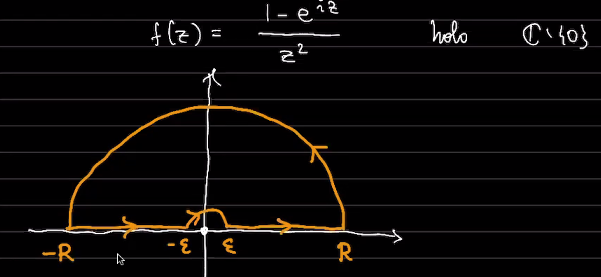
\includegraphics[width=250px]{C:/Users/Alex/Desktop/Notes/Spring 2021/pics/indentedsemicirclecontour.PNG}

	In the limit we'll get what we want. Note integral is 0 to start. So suffices to compute another integral along different path

	\begin{align*}
		\int_{\gamma_{\epsilon}} \frac{1-e^{iz}}{z^2}dz = \int_{\gamma_{\epsilon}} \frac{-iz + g(z)}{z^2}dz = \int_{\gamma_{\epsilon}} \frac{-i}{z}dz = - \pi
	\end{align*}

	where $g(z)$ is remainder of power series which is holomorphic. Value of the integral comes from the singularity
\end{prop}
\begin{theme}
	Note we used linearity of the integral + the powerseries to make integration easier, and recover a holomorphic function(which is often made nonholomorphcic by singularities 1/z)
\end{theme}

\begin{theorem}
	Suppose f is holomorphic in an open set that contains the closure of a disc D. If C denotes the boundary circle of this disc with the positive orientation, then
	\begin{align*}
		f(z) = \frac{1}{2 \pi i} \int_C \frac{f(\zeta)}{\zeta - z}d \zeta
	\end{align*}

	for any point in closure of disc D.
\end{theorem}

\begin{proof}
	Fix $z \in D$ and consider with keyhole $\Gamma_{\delta,\epsilon}$, omitting z. 

	Clearly $\int_{\Gamma_{\delta,\epsilon}} F(\zeta) d\zeta = 0$ since holomorphic away from singularity. We let $\delta \to 0$ and use continuity of F to see the limit the integrals of corridors cancel. 

	$F(\zeta) = \frac{f(\zeta) - f(z)}{\zeta - z} + \frac{f(z)}{\zeta  - z}$ this give us the result in the limit.

	The key is to use holomorphicity to rewrite expression and then factor out an $f(z)$. 

\end{proof}

\begin{prop}
	If f is holomorphic in an open set $\Omega$, the f has infinitely many complex derivatives in $\Omega$. Moreover if $C \subseteq \Omega$ is a circle whose interior is also contained in $\Omega$ then
	\begin{align*}
		f^{(n)}(z) = \frac{n!}{2 \pi i} \int_C \frac{f(\zeta)}{(\zeta - z)^{n+1}}
	\end{align*}
\end{prop}

\begin{prop}
	Cauchy's Inequalities: If f is holomorphic in an open set that contains the closure of disc D centered at $z_0$ and of radius R, then
	\begin{align*}
		|f^{(n)}(z_0)| \leq \frac{n!}{R^n}||f||_C
	\end{align*}
\end{prop}

\begin{theorem}
	\textit{Rigidity}: If $f : \Omega \to \C$ holomorphic, and has $z_n$ which converges in $\Omega$ to $w$, with all $f(z_n) = 0$. Then f = 0
\end{theorem}

\begin{proof}
	First we show f 0 near w. 

	Use power series expansion. AFSOC not 0 near w. Then we have an $a_n \neq 0$. Take minimal one. Compute $f(z) = a_m(z-w)^m(1+g(z))$ where g holomorphic. But as we take a point close enough, we know $f(z_n)$ should be 0 but the product above cannot be. So done in a set

	Let $U = int\{z: f(z) = 0\}$. We know U nonempty. U open, but U also closed because f continuous. Furthermore we can find a neighborhood around z in U(by first part). So it must be U everything since U connected. 
\end{proof}

\begin{theorem}
	Morera's Theorem:
	If cts f vanishes on triangles then it's holomorphic. 
\end{theorem}

\begin{proof}
	We know we can find a primitive via the proof of cauchy's theorem. Further it's holomorphic. Then f is holomorphic. 
\end{proof}

\begin{prop}
	Uniqueness of analytic continuation. If two holomorphic f,g equal on sequence of points then equal everywhere.
\end{prop}

\begin{proof}
	True by regularity(look at difference). 
\end{proof}

\begin{quest}
	When is there a continuation?
\end{quest}

\begin{ans}
	There should only be a problem at boundary(can think of compact functions going to 0).
\end{ans}

\begin{remark}
	Miracles of holomorphicity: Closedness, regularity, unique extension(rigidity).
\end{remark}

\begin{theorem}
	Morera's Theorem: Converse to cauchy's theorem.

	Suppose $f$ cts on $f : D \to \C$ s.t. for all triangles we have 0 then f holomorphic.
\end{theorem}

\begin{proof}
	From cauchy we know we have $F$ holo on D with $F' = f$.(via this triangle property). Since F holomorphic then f holomorphic. 
\end{proof}

\begin{prop}
	Uniform limits of holo. functions are holo
\end{prop}

\begin{proof}
	If we can show the limit vanishes on triangles then done by Morera. Note we know unif. limits of cts functions are cts. But this is clear just from DCT.
\end{proof}

\begin{remark}
	Recall this does not hold in real case: think weierstrass's theorem(polynomials can uniformly approximate any cts function).
\end{remark}

\begin{theorem}
	Derivative of limit is limit of derivatives of holo. function
\end{theorem}

\begin{proof}
	We go for a bound on the derivative in terms of f: $||F'||_{\infty,\Omega_{\delta}} \leq \frac{1}{\delta}||F||_{\infty,\Omega_{\Omega}}$. This is enough when we look at diferences of the derivatives(take out limit)

	We go by cauchy's formula:
	\begin{align*}
		|F'(z)| = |\frac{1}{2\pi i}\int_{\partial D_{\delta}(z)}\frac{F(w)}{(w-z)^2}dw|
	\end{align*}

	and apply triangle inequality
\end{proof}

\begin{remark}
	True for higher order derivatives. Amazing that knowing holomorphicity gives control of limit of all derivatives. 
\end{remark}

\begin{theme}
	Constructing holomorphic functions: look at series of holomorphic functions(assuming unif. convergence on compact sets)

	Also often useful to define as integrals of holomorphic functions of a parameter.
\end{theme}

\begin{prop}
	Let $F : \Omega \times [0,1] \to \C$. be s.t. 

	i) $z \to F(z,s)$ is holo. for all s

	ii) F cts on $\Omega \times [0,1]$. Then 

	$f(z) = \int_0^1 F(z,s) ds $
\end{prop}

\begin{proof}
	We argue the integral is the uniform limit of the riemanns sums. 

	Write $f_n(z) = \frac{1}{n}\sum^n F(z,k/n)$. Uniform bound comes from continuity: cause we're on a comapct set
\end{proof}

\begin{theorem}
	\textit{Reflection Principle}: Let $\Omega \subseteq \C$ sym. about $\R$. Let $\Omega^+$ be part above real line. Let I be real part. 

	\textit{Symmetry Princple:} Let $f^{+/-}: \Omega^{+/-} \to \mathbb{C}$ holo, both extend cts to I(maybe not holomorphcally). And extensions agree. Then gluing everyting together we get f a holomorphic function. 

	
\end{theorem}

\begin{proof}
	Simply need to check boundary. After showing continuity use morera's theorem(converse to gousard). 

	Hardest case is triangle over interval. Then we simply subdivide and integrate each function along restricted sub-divisions. We use continuous extension by shifting triangles down by $\epsilon$. 
\end{proof}

\begin{remark}
	Real line is irrelevant, can be any curve. Also note holomorphicity is extended by continuity.
\end{remark}

\begin{theorem}
	Schwarz Refletion Principle: Let $f^+: \Omega^+ \to \mathbb{C}$ holo, $f^+$ extends cts to I, $f|_I \in \mathbb{R}$ and reflecting over it.
\end{theorem}

\begin{proof}
	Define $f^-$ and argue using reflection. Set $f^-(z) = \overline{f(\overline{z})}$. Simply need to check holomorphicity(since agreement on real line). 

	To show holo. we use power series. Note bar distributes over multiplication and we're done.
\end{proof}
	
\begin{theorem}
	\textit{Runge's Theorem}: Let $K \subseteq \mathbb{C}$ with f holo. in neighborhood of K. Then f can be approximuated uniformly by rational functions with singularities in $K^C$. 

	If $K^C$ connected then the rational functions can be polynomials. 
\end{theorem}

\begin{proof}
	Use cauchy's formula plus riemann sums. 

	Connectedness(in $K^C$) is used to push away singularities.
\end{proof}

\begin{example}
	$e^{1/z}$ has essential singularity at 0(blows up faster than any rational function at 0). 
\end{example}

\begin{remark}
	We can locally write $f(z) = (z-z_0)^n g(z)$ for a zero $z_0$ of f for g nonvanishing locally.
\end{remark}


\end{document}

